\chapter{\kadaic}
\section{\purpose}
\paragraph{方位残効とは}
方位残効とは,ある方向に傾いた線分を眺めて順応した後,テスト垂直の線分を見ると,順応刺激と反対の方向に傾いて知覚される現象である\cite[p.5]{方位残効と運動残効のメカニズム}.
\paragraph{方位選択性とは}
大脳皮質視覚野細胞は受容野に特定の傾き(方位)線分刺激を提示したときに応答し,それと異なる傾きの刺激には応答しないことを,方位選択性という\cite[p.764]{方位選択性}.
\paragraph{目的}今回の実験では,方位の大きさと,残効の度合いを比較し,視覚情報処理を考慮したうえで,現象について考察する.
\section{\method}
\paragraph{\kadaica}
方位を定義できる正弦波縞を作成する.
方位\(\theta\),空間周波数\(f\),コントラスト\(C\)の正弦波縞は\eqref{equ:正弦波縞}で表せる.
\(L(x,y)\)を点\(L(x,y)\)における輝度,\(L_0\)を全体画像の平均輝度とする.
\begin{align}
    L(x,y) & = L_0\Bigg(1+C\sin\Big(2\pi f\big(y\sin(\theta)+x\cos(\theta)\big)\Big)\Bigg)\label{equ:正弦波縞}
\end{align}
\(y\)軸方向を基準とし,
左に\(30^\circ\)傾いた空間周波数\(0.05\textrm{cycle}/\textrm{pixel}\)の正弦波縞と,
右に\(60^{\circ}\)傾いた空間周波数\(0.03\textrm{cycle}/\textrm{pixel}\)の正弦波を作成する.
平均輝度は,最大輝度の\(0.5\)倍,コントラストを\(0.5\)とする.
\paragraph{\kadaicb}
方位\(90\pm 10^\circ\),\(90\pm 45^\circ\)正弦波縞の順応刺激を上下に提示して,\(60\)秒後に垂直縞\(90^\circ\)のテスト刺激を表示する.
全体画像サイズを\(\textrm{縦}900\times\textrm{横}400\textrm{pixel}\),格子縞のサイズを\(400\times 400\textrm{pixel}\),順応時に提示する中央の矩形を\(20\times 100\textrm{pixel}\),順応後の注視点を\(20\textrm{pixel}\)とする.
正弦波縞の空間周波数を\(0.03\textrm{cycle}/\textrm{pixel}\),コントラストは\(0.5\)とする.
刺激を観察する際,網膜上の,局所的な明るさの順応を避けるために,\(60\)秒の順応時間では,矩形を満遍なく見るようにする.
\begin{flushright}
    \vspace{-1em}
    \begin{minipage}[t]{.48\textwidth}
        \begin{lstlisting}[caption={矩形と円の作成},label={src:矩形と円の作成}]
[w, h] = meshgrid(-199:200, 50:-1:-49);
Y2 = 255*0.95;
cir = (w.^2 + h.^2 >= 10.^2)*Y2; % 円
rct = ones(100,400); % 矩形
rct = rct * Y2;
rct(50-9:50+10,200-49:200+50)=0;
        \end{lstlisting}
    \end{minipage}
    \hspace{.5em}
    \begin{minipage}[t]{.48\textwidth}
        \begin{lstlisting}[caption={順応刺激画像の作成},label={src:順応刺激画像の作成}]
% L: 正弦波縞 90°
% L_p10,L_n10: 正弦波縞 ±10° 
% L_n45,L_p45: 正弦波縞 ±45°
dg_90 = [L; cir; L];
dg_10 = [L_p10; rct; L_n10];
dg_45 = [L_n45; rct; L_p45];
        \end{lstlisting}
    \end{minipage}
    \vspace{-.5em}
\end{flushright}

\begin{wrapfigure}{r}[-1mm]{.48\textwidth}
    \vspace{-1cm}
    \begin{lstlisting}[caption={刺激画像の表示方法},label={src:刺激画像の表示方法}]
fig = figure;
set(fig, 'position',get(0,'ScreenSize'));
colormap(gray(256));
image(dg_10);
axis off;
axis image;    
    \end{lstlisting}
    \vspace{-1cm}
\end{wrapfigure}
\paragraph{刺激画像の表示}
順応刺激画像を方位残効が生じやすいように,全画面表示にし,\(60\)秒後にテスト刺激を提示するためには,\matlab の\texttt{set}関数を用いる.
また,\(60\)秒の待機時間を\texttt{pause(60)}で設定する.画像に軸や数値ラベルを表示しないために,\texttt{axis}も設定する.
\section{\result}
\begin{figure}[h]
    \centering
    \begin{minipage}[b]{.19\textwidth}
        \centering
        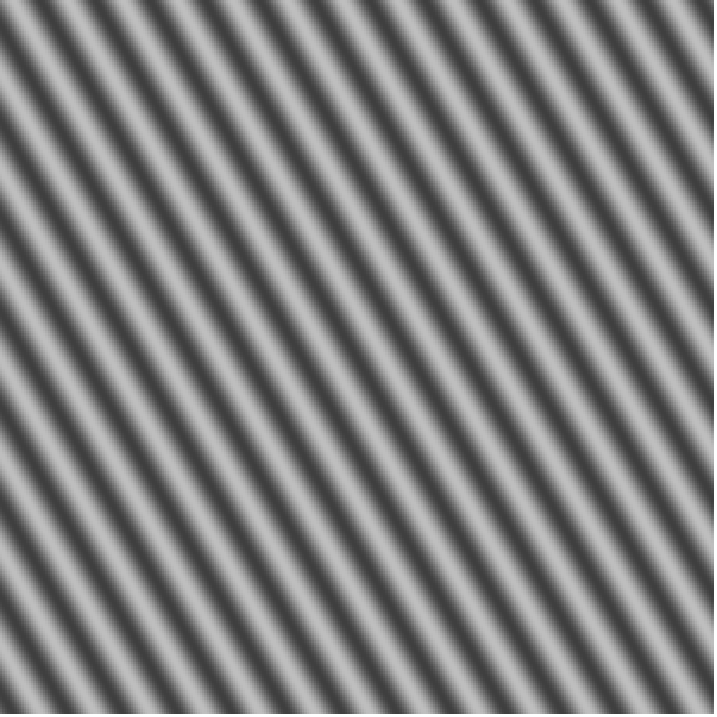
\includegraphics[keepaspectratio,width=\textwidth]{../../Figures/07_10_l30.pdf}
        \subcaption{左に\(30^\circ\)}
    \end{minipage}
    \begin{minipage}[b]{.19\textwidth}
        \centering
        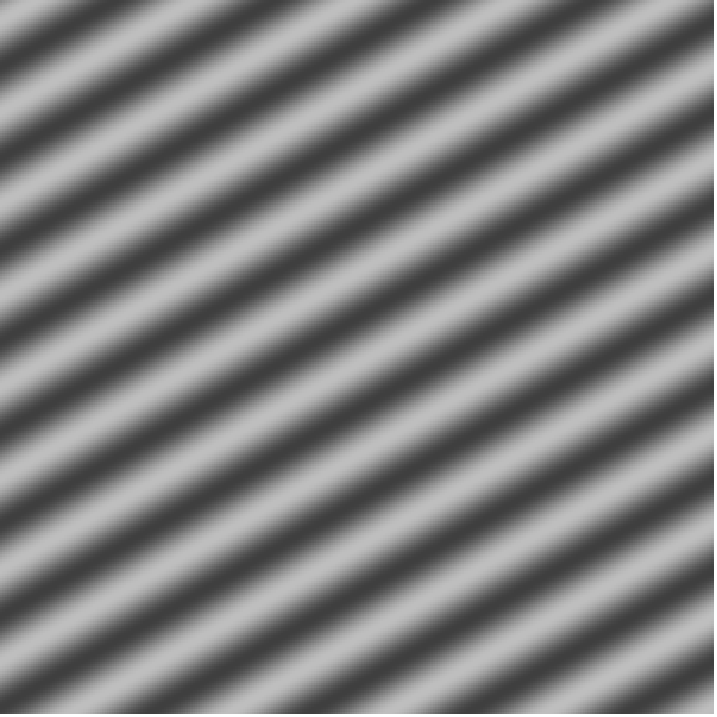
\includegraphics[keepaspectratio,width=\textwidth]{../../Figures/07_11_r60.pdf}
        \subcaption{右に\(60^\circ\)}
    \end{minipage}
    \begin{minipage}[b]{.19\textwidth}
        \centering
        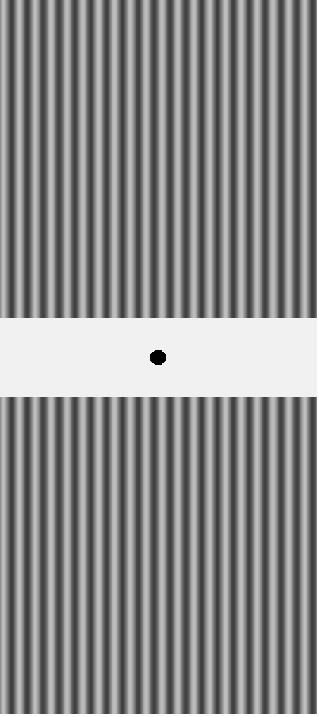
\includegraphics[keepaspectratio,width=.6\textwidth]{../../Figures/07_21_dg90.pdf}
        \subcaption{テスト刺激}
    \end{minipage}
    \begin{minipage}[b]{.19\textwidth}
        \centering
        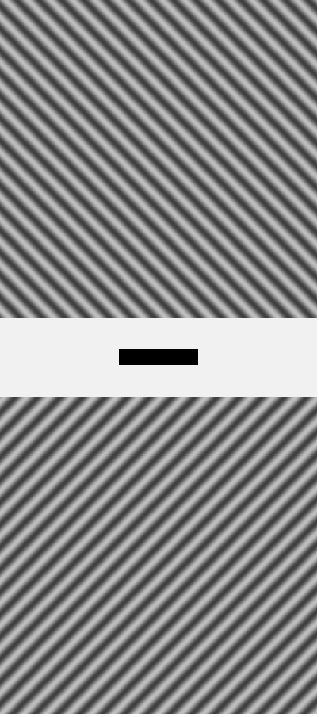
\includegraphics[keepaspectratio,width=.6\textwidth]{../../Figures/07_22_dg45.pdf}
        \subcaption{順応刺激\ \(90\pm 45^\circ\)}
    \end{minipage}
    \begin{minipage}[b]{.19\textwidth}
        \centering
        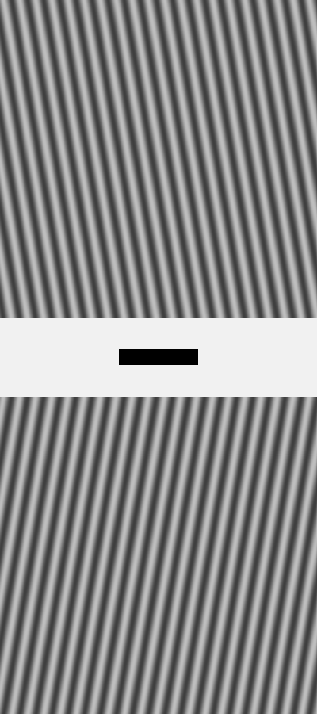
\includegraphics[keepaspectratio,width=.6\textwidth]{../../Figures/07_23_dg10.pdf}
        \subcaption{順応刺激\ \(90\pm 10^\circ\)}
    \end{minipage}
    \caption{生成した画像}
\end{figure}
\paragraph{方位残効}
順応刺激\(90\pm10^\circ\)は,方位残効を知覚できた.順応刺激\(90\pm45^\circ\)は,方位残効を知覚できなかった.
\section{\consideration}
